\chapter{Classification of symmetrical windings}
This report\footnote{Text taken from \cite{REF-00014}.} is devoted to a derivation of an algorithmic method to design $m$-phase symmetrical windings and a representation thereof in a compact form. The basic principle of the winding of an electrical machine is to obtain a rotating magnetic field in the stator (the stationary part) that interacts with the moving part (the rotor). This is achieved by arranging the coils of the winding in the stator slots around the air gap periphery in such a way that a rotating field is developed when applying currents. As a result the induced voltage, which arises from flux per pole $\hat{\Phi}$, is obtained from Faraday's law. In general the sinusoidally induced voltage for a winding having $N_s$ series turns per phase is
\begin{equation}
  \label{eqn:ui}
  U_i = \sqrt{2} \pi f_1 \xi_p N_s \hat{\Phi}, \qquad \xi_p \leq 1
\end{equation}
where $\xi_p$ is the winding factor of the \textit{working harmonic}. The induced voltage in \eqref{eqn:ui} brings the importance of the winding design to the fore. For a given design requirement, it is desirable to have $\xi_p$ as high as possible.

\section{Definition of the working harmonic}\label{sec:working_harmonic}
Throughout the analysis all harmonics are referred to in terms of the bore $2\pi$ of the machine, i.e.~the \textit{fundamental harmonic} has the order $\nu=1$ and forms one pole pair. The harmonic that produces the magnetic field that interacts with the rotor poles $2p$ has the order $\nu=p$ and is called the \textit{working harmonic}. Any other harmonic of the $\nu^{th}$ order will have $\nu$ pole pairs and spans a peripheral angle of $\frac{2\pi}{\nu}$.
\index{working harmonic}

Often the harmonic orders are normalised with respect to the \textit{working harmonic}, i.e.~$\xi_{\nu /p}$. This then means that the \textit{working harmonic} is written as $\xi_1$ and sub-harmonics will have a fraction as subscript. This notation will not be used in this report.

\section{Basic winding properties}%
\label{sec:m_phases}
The winding design can be quite a difficult task and at this point it is useful to have a coarse classification of symmetrical windings. Since symmetrical windings comprise such a great variety, an attempt to categorise them will depend on the properties by which they are to be sorted. 

\subsection{Slots and coils per pole and phase} \label{subsec:slots_coils}
Any $m$-phase winding could be characterised by its number of slots per pole and phase. However, when comparing different winding designs with each other this number alone is insufficient. It does not take into account the number of layers the winding has. In addition, the number of coils per pole and phase should be defined. For a machine with $Q_s$ stator slots, $p$ pole pairs and $m$ phases the following definitions holds:

\begin{defth}
Slots per pole and phase: 
\begin{equation}
  q =\frac{Q_{s}}{m2p}=\frac{q_{n}}{q_{d}}
\end{equation}
$\frac{q_{n}}{q_{d}}$ is the reduced form of $q$. Each phase has $q_n$ slots that are distributed over $q_d$ poles. In the case where $q_d$ equals one, $q$ is an integer and the winding is called an integer slot winding. When $q_d$ is greater than one, it is called a fractional slot winding. 
\end{defth}
\begin{defth}
Coils per pole and phase: 
\begin{equation}
  q_{c}=\frac{Q_{c}}{m2p}=\frac{q_{c_n}}{q_{c_d}}
\end{equation}
$\frac{q_{c_n}}{q_{c_d}}$ is the reduced form of $q_c$. Each phase has $q_{c_n}$ coils distributed over $q_{c_d}$ poles. If $q_{c_n}$ is greater than one and $q_c$ is not equal to one it is a distributed winding. 
\end{defth}
These characteristic numbers give useful information on the winding when they are written as a reduced improper fraction\footnote{The reduced fraction could be either a proper or an improper fraction. An improper fraction has the numerator greater than the denominator.}. Additionally, the properties of single and double layer windings are summerised in Tab.~\ref{tab:properties_single_double}. 
\index{slots per pole and phase}
\index{reduced form}
\index{coils per pole and phase}

{\renewcommand{\arraystretch}{1.2}
\begin{table}[htbp]
  \caption{Winding properties}
  \label{tab:properties_single_double}
  \centering
  \begin{tabular}{|c|c|}
  \hline
  single layer winding & double layer winding \\
  \hline
  $q = 2q_c$ & $q = q_c$ \\
  $Q_s = 2Q_c$ &  $Q_s = Q_c$ \\
  \hline
  \end{tabular}
\end{table}}
\index{winding properties}

\subsection{Average coil pitch}
The coil pitch is defined as the peripheral angle between the two coil sides. It is practical to express the coil pitch in terms of the number of slots. Therefore, it is an integer number. 
\begin{defth}
The average coil pitch is defined as
\begin{equation}
  \label{eqn:y_p}
  y_p = \frac{Q_s}{2p}
\end{equation}
and the implemented coil pitch is given by
\begin{equation}
  \label{eqn:y_d}
  y_d = \mbox{int}(y_p)\pm k
  \quad
  \begin{cases}
    k \in \mathbb{N} \\
    y_d \geq 1
  \end{cases}
\end{equation}
\end{defth}
In the case where $y_d=y_p$ it is a full-pitch winding. If $y_d \neq y_p$ it is called a fractional pitch winding. 
\index{average coil pitch}

\subsection{Classification scheme}
The aim of the classification scheme is to find a way to relate different winding types to each other. It is also a useful guideline to compare windings that belong to the same category. For the design methodology offered in this report, the following winding parameters are chosen for the classification:
\begin{enumerate}
  \item the reduced form of the number of coils per pole per phase;
  \item the average coil pitch; and 
  \item the number of layers.
\end{enumerate}
Tab.~\ref{fig:classification} shows a possible way to classify symmetrical $m$-phase windings. The reason for choosing the average coil pitch as a second property arises from the construction of the coils and it is valid for all types of windings. It could be seen as the ideal coil pitch. Additionally, the number of layers is a key parameter since the technology for manufacturing and the material used in single layer windings are different from that used in double layer windings. Using this classification scheme, the following definitions are associated with windings:
\begin{description}
  \item[Distributed winding:] If the numerator $q_{cn}$ of $q_c$ is greater than~%
  one, the winding is distributed. This means that the coil sides are distributed~%
  over $q_{cn}$ slots. The opposite of a distributed winding is a concentrated~%
  winding.
  \item[Concentrated winding:] In the case where $q_{c_n}$ equals one, it is called~%
  a concentrated winding. 
  \item[Concentrated coil:] When $y_d$ equals one, it is a concentrated coil. In~%
  this case the coil is concentrated around a stator tooth.
  a concentrated winding. 
  \item[Single and double layer:] These windings are differentiated by the number~%
  of coils compared to the number of stator slots. In single layer windings the~%
  number of coils equals half the number of stator slots, while for double layer~%
  windings the number of coils is equal to the number of stator slots. In the~%
  present dissertation a double layer winding has two coil sides per slot which could~%
  placed radially in two layers or side by side. 
  \item[Overlapping and non-overlapping:] In overlapping windings the coils overlap~%
  and the coil pitch $y_d$ is greater than one. If the coil pitch $y_d$ equals one,~%
  the coils do not overlap.
  \item[Integral slot winding:] If the denominator $q_d$ equals one, the phase~%
  belt has $q_n$ slots over one pole.
  \item[Fractional slot:] The denominator of $q$ is greater than one. This~%
  means that the $q_n$ slots are distributed over $q_d$ poles. In addition,~%
  the average coil pitch $y_p$ is a fraction. 
\end{description}
{\renewcommand{\arraystretch}{1.2}
\begin{table}[htbp]
  \centering
  \caption{Classification of symmetrical windings}
  \label{fig:classification}
  \begin{tabular}{|l|l|l|}
  \hline
  Parameter  & Constraint  &  Classification  \\
  \hline
  \multirow{2}{*}{$Q_c$} & $\frac{1}{2}Q_s$ & single layer \\
                         & $Q_s$            & double layer \\
  \hline                        
  \multirow{2}{*}{$y_d$} & $=1$  & non-overlapping         \\
                         & $>1$  & overlapping             \\
  \hline                         
  \multirow{2}{*}{$y_d$} & $=y_p$     & full-pitch         \\
                         & $\neq y_p$ & fractional pitch   \\
  \hline                         
  \multirow{2}{*}{$q_d$} & $=1$     & integral slot        \\
                         & $>1$     & fractional slot      \\
  \hline                         
  \multirow{2}{*}{$q_{c_n}$} & $=1$     & concentrated     \\
                             & $>1$     & distributed      \\  
  \hline
  \end{tabular}
\end{table}}

It is important to distinguish between a concentrated winding and a concentrated coil. The classification scheme in Fig.~\ref{fig:classification} defines a concentrated winding in a unique way. Concentrated windings are defined differently in literature. \cite{REF-00814} refers to it as a traditional single layer winding whereas \cite{REF-00822} refers to it as distributed.
\index{concentrated winding}
\index{concentrated coil}
\index{classification scheme}
\index{distributed winding}

Particularly the windings defined as a fractional slot are very attractive for use in permanent magnet synchronous machines. Especially the single layer non-overlapping winding could be used to reduce (a) manufacturing costs compared to overlapping windings; (b) the end winding losses; (c) torque ripple; and (d) the mutual coupling between the phases.
\index{manufacturing costs}
\index{end winding losses}
\index{torque ripple}
\index{mutual coupling}

\section{Characteristics of symmetrical windings}
This section contains the major properties by which symmetrical $m$-phase windings are characterised.

\subsection{Basic winding}
\begin{defth}
The smallest repetitive segment is called the basic winding (German: ``Urwicklung'').
\end{defth} 
Due to symmetry only the basic winding needs to be determined. If $q_d$ is less than $p$ the winding is composed of $t$ identical \textit{basic windings}, i.e.
\begin{equation}
  \label{eqn:gcd_t}
  \begin{array}{ll}
  t = \begin{cases}
        \gcd\left(Q_s,p\right)  & \text{for double layer}\\
        \gcd\left(\frac{Q_s}{2},p\right) & \text{for single layer}
      \end{cases}
  \end{array}
\end{equation}
and gcd is called the greatest common divisor. In the case where $t=1$ the winding has no symmetry. Each of the $t$ \textit{basic windings} will have $Q_b$ slots and $p_b$ pole pairs, therefore
\begin{equation}
  \label{eqn:qd_pb}
  Q_b = \frac{Q_s}{t} \quad \mbox{and} \quad p_b = \frac{p}{t} 
\end{equation}
The number $p_b$ is the reduced pole pair. Another way of obtaining this number is by means of the denominator of $q_c$, i.e.
\begin{equation}
  \label{eqn:p_b}
  p_b =  
  \begin{cases}
    \frac{1}{2} q_{c_d}  & q_{c_d} \: \textnormal{even} \\
    q_{c_d}  & q_{c_d} \: \textnormal{odd}
  \end{cases}
\end{equation} 
which is independent of $t$. Examining \eqref{eqn:gcd_t}, it is recognised that $t$ can be rewritten as the gcd between the number of coils and the pole pairs, i.e.
\begin{equation}
  \label{eqn:gcd_t_gcd(Qc_p)}
  t = \gcd(Q_c,p) \quad
  \begin{cases}
    Q_c = Q_s \quad & \textnormal{double layer} \\
    Q_c = \frac{1}{2}Q_s \quad & \textnormal{single layer}
  \end{cases}
\end{equation} 
which is valid for both single and double layer windings. Although $t$ is usually used as a variable for time it is commonly found in literature and will be used in the same way throughout this chapter. Since the winding design is independent of time, it does not cause any confusion.

It is favourable to use the terms ``in and out going coil sides''\footnote{This is similar to the current which is defined as into and out of the page.}. Only the in going coil side needs to be assigned\footnote{The use of coil sides are preferred above coils, since it is then independent whether the coil sides belong to the same coil or not.} since the out going coil side is given by the coil pitch and type of winding.

\subsection{Winding symmetry}
For a winding to be symmetrical the number of coils used in each of the phases must be equal. Therefore the quotient between $Q_c$ and $m$ must be an integer. A requirement for a winding to be symmetrical can be derived from \eqref{eqn:qd_pb}. The symmetry condition can be expressed as
\begin{equation}
  \label{eqn:feasibility}
  \frac{Q_s}{t} = mk, \quad  k \in  \mathbb{N}
\end{equation}
which relates the pole number, number of stator slots and phase number to each other. A very useful function employed in the method is the modulo function which finds the remainder after division, i.e.~ $\textnormal{mod}(a,b)=a-\textnormal{floor}(\frac{a}{b})$\footnote{The floor function of a real number $x$, floor($x$), is a function whose value is the largest integer less than or equal to $x$.}. When using the modulo function it means that $\textnormal{mod}(\frac{Q_s}{t},m)$ must equal zero. There are different ways of deriving the constraints for the winding symmetry condition. Tab.~\ref{tab:feasibility} gives different variations found in the literature to express the symmetry condition. 
{\renewcommand{\arraystretch}{1.6}
\begin{table}[h]
  \caption{Constraints for symmetry}
  \label{tab:feasibility}
  \centering
  \begin{tabular}{|l|l|}
  \hline
  Reference & Constraint \\
  \hline
  \multirow{2}*{\cite{REF-00452}} & $\gcd(q_{c_d},m)=1$  \\
  &$\mbox{mod}\bigl(\frac{Q_c}{q_{c_n}}q_{c_d},m\bigr)=0$\\
  \hline
  \cite{REF-00754} & $\mbox{mod}\bigl(\frac{Q_s}{\gcd(Q_s,2p)},m\bigr)=0$  \\
  \hline
  \cite{REF-00486} & $\mbox{mod}\bigl(\frac{Q_s}{t},m\bigr)=0$ \\
  \hline
  \end{tabular}
\end{table}}

\subsection{Reduced number of pole pairs}
The lowest harmonic generated by a winding is given by $t=\gcd\left(Q_c,p\right)$ and the working harmonic equals $p$. The reduced pole number gives information on the sub-harmonics which are summarised as follows:
\begin{equation}  
 \begin{aligned}
  t &= p \quad \textnormal{the winding has no sub-harmonics} \\
  t &< p \quad \textnormal{the winding has sub-harmonics}
  \end{aligned}
\end{equation} 

The reduced number of pole pairs can be calculated in two different ways. Two greatest common divisors, i.e.~$\gcd\left(Q_c,2\,m\,p\right)$ and $\gcd\left(Q_c,p\right)$, are used to get $q_{c_d}$ and $p_b$ respectively. The relationship between these two factors is as follows:
\begin{equation}
  \label{eqn:reduced_p} 
  \gcd\left(Q_c,p\right)=\frac{\gcd\left(Q_c,2\,m\,p\right)}{r} \hspace{15pt}
  \textnormal{where} \hspace{15pt} r=
  \begin{cases}
   m  & \text{$q_{c_d}$ even}\\
   2m & \text{$q_{c_d}$ odd}
  \end{cases}
\end{equation}

\section{Rotating mmf}
Distributing the coils around the air gap periphery firstly requires the winding characteristic as explained in section \ref{subsec:slots_coils} and secondly a constraint assuring that the coils are assigned uniquely to the stator slots. Deriving such a constraint is done by means of the magnetomotive force (mmf) produced by a winding. 
\index{magnetomotive force}

In the theory of three-phase windings the rotating magnetic field is derived from a single coil with $N_t$-turns. The mmf produced by the coil is then written as a Fourier series which allows it to be decomposed in the \textit{working harmonic}, higher order harmonics and sub-harmonics if applicable. A detailed mathematical derivation is given by \cite{REF-01043}. It is also possible to explain the decomposition by means of visualisation as shown in \cite{REF-00004}, \cite{REF-00294} and  \cite{REF-00330}. The visualisation method is preferred and is used in the next sections in order to define the mmf envelope functions. This is necessary to answer the research sub-question which is the mathematical expression that defines a phase belt.
\index{harmonics}
\index{sub-harmonics}

\subsection{The mmf of a single turn coil}%
\label{subsec:nt-turn_coil}
Consider a single coil with $N_t$-turns carrying a current $i$ placed in the stator of a machine with a uniform air gap as shown in Fig.~\ref{fig:mmf_1}\subref{fig:sincol}. Assuming an infinite permeability in the laminated parts, the mmf in the stator and rotor can be neglected. This means the mmf across the air gap will be equal to the total mmf. 
 
\begin{figure}[htbp]
  \centering
  \fontsize{8}{10}\selectfont
  \subfloat[Single coil\label{fig:sincol}]{
  \begin{psfrags}%
\psfragscanon

% text strings:
\psfrag{x01}{$0$}
\psfrag{x02}{$\frac{\pi}{3}$}
\psfrag{x03}{$\frac{2\pi}{3}$}
\psfrag{x04}{$\pi$}
\psfrag{x05}{$\frac{4\pi}{3}$}
\psfrag{x06}{$\frac{5\pi}{3}$}
\psfrag{x07}{$2\pi$}

\psfrag{t01}{-1}
\psfrag{t02}{+1}
\psfrag{t03}{$C_2$}
\psfrag{t04}{$C_1$}
\psfrag{t05}{$F$}
\psfrag{t06}{$\frac{4}{\pi}\frac{N_ti}{2}\sum\limits_{\nu=1}^{\infty}
            \frac{1-(-1)^{\nu}}{2} \frac{1}{\nu}\cos(\nu \theta)$}
\psfrag{t07}[br]{$\theta$}
\psfrag{t08}{$\mu \rightarrow \infty$}
\psfrag{t09}{magnetic}
\psfrag{t10}{axis}
\psfrag{t11}{$p_1$}
\psfrag{t12}{$\theta^{+}$}
\psfrag{t13}{$\frac{4}{\pi}\frac{N_ti}{2}\cos \theta$}
\psfrag{t14}{current sheet}
\psfrag{t15}{$N_t i$}
\psfrag{t16}{$C_3$}
\psfrag{t17}{(a)}
\psfrag{t18}{(b)}
\psfrag{t19}{$\delta$}

% Figure:
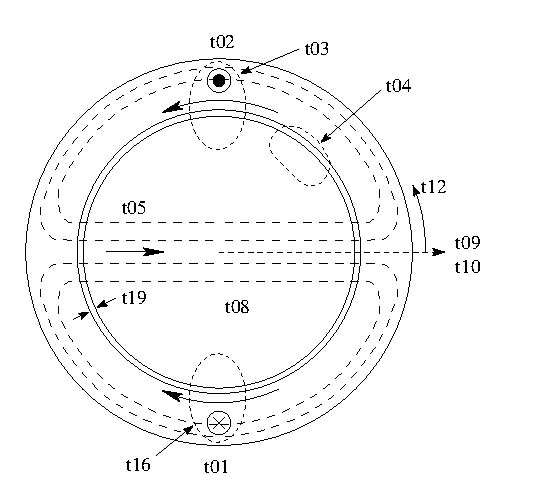
\includegraphics[height=5.5cm]{figs/f_mmf_1a.eps}
\end{psfrags}%}
  \hfill
  \subfloat[Spatial mmf distribution\label{fig:spatmmf}]{
  \begin{psfrags}%
\psfragscanon

% text strings:
\psfrag{x01}{$0$}
\psfrag{x02}{$\frac{\pi}{3}$}
\psfrag{x03}{$\frac{2\pi}{3}$}
\psfrag{x04}{$\pi$}
\psfrag{x05}{$\frac{4\pi}{3}$}
\psfrag{x06}{$\frac{5\pi}{3}$}
\psfrag{x07}{$2\pi$}

\psfrag{t01}{-1}
\psfrag{t02}{+1}
\psfrag{t03}{$C_2$}
\psfrag{t04}{$C_1$}
\psfrag{t05}{$F$}
\psfrag{t06}{$\frac{4}{\pi}\frac{N_ti}{2}\sum\limits_{\nu=1}^{\infty}
            \frac{1-(-1)^{\nu}}{2} \frac{1}{\nu}\cos(\nu \theta)$}
\psfrag{t07}[br]{$\theta$}
\psfrag{t08}{$\mu \rightarrow \infty$}
\psfrag{t09}{magnetic}
\psfrag{t10}{axis}
\psfrag{t11}{$p_1$}
\psfrag{t12}{$\theta^{+}$}
\psfrag{t13}{$\frac{4}{\pi}\frac{N_ti}{2}\cos \theta$}
\psfrag{t14}{current sheet}
\psfrag{t15}{$N_t i$}
\psfrag{t16}{$C_3$}
\psfrag{t17}{(a)}
\psfrag{t18}{(b)}
\psfrag{t19}{$\delta$}

% Figure:
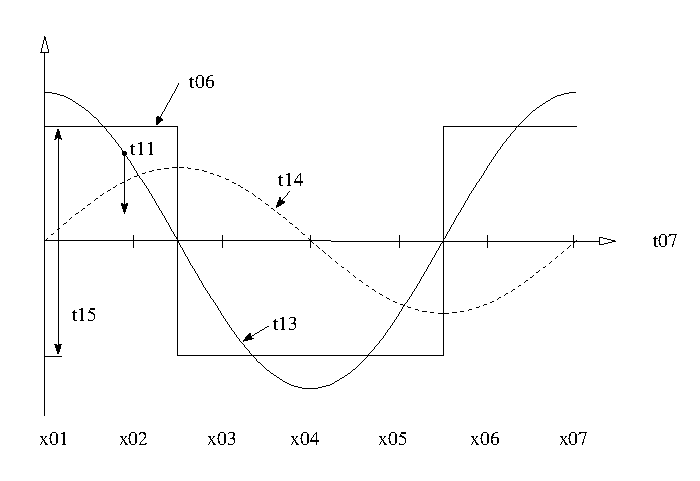
\includegraphics[height=5.5cm]{figs/f_mmf_1b.eps}
\end{psfrags}%}
  \caption{Single $N_t$-turn coil}
  \label{fig:mmf_1}
\end{figure}

The spatial mmf distribution around the air gap periphery is obtained by applying Amp\`ere's law to the contours $C_1$, $C_2$ and $C_3$. The results of the integration are given in \eqref{eqn:int_H}. The integral along $C_1$ is zero since the contour does not enclose any source. Contrary to this the integrals along $C_2$ and $C_3$ equal $N_ti$ and $-N_ti$ respectively. The current in coil side $+1$ is positive, and using the right hand rule, out of the page.  
\begin{equation}
 \label{eqn:int_H}
 \oint \vec{H} \cdot d\vec{l}=
 \begin{cases}
   \begin{array}{llll}
     0  & C_1 & 0 \leq \theta < \frac{\pi}{2} 
     & \Rightarrow H(0)=H(\theta_1)\\
     N_ti & C_2 & \frac{\pi}{2} \leq \theta < \frac{3\pi}{2} 
     & \Rightarrow H(0)-H(\theta_2) = \frac{N_ti}{\delta} \\
     -N_ti & C_3 & \frac{3\pi}{2} \leq \theta < \frac{5\pi}{3} 
     & \Rightarrow H(0)-H(\theta_3) = \frac{N_ti}{\delta}
   \end{array}
 \end{cases}
\end{equation}
Since the flux to and from the rotor are equal, the air gap mmf will have an amplitude of $\frac{N_ti}{2}$. Fig.~\ref{fig:mmf_1}\subref{fig:spatmmf} shows the spatial of the single coil. This is a square wave and from the Fourier series the fundamental has an amplitude of $\frac{4}{\pi}$. The fundamental mmf can be seen as the result of a sinusoidally distributed current sheet on the stator inner diameter. When the coil is supplied by a current 
\begin{equation}
  i = \hat{I}\cos\omega t
\end{equation}
any point on the mmf will have a vertical trajectory. For example, the point $p_1$ will start moving downward for $t^+$ until it reaches a minimum from where it will start to move upwards again. Applying a sinusoidal current to the coil results in a standing wave in the air gap. The spatial mmf distribution has the form
\begin{equation}
  \label{eqn:F_theta_t_1}
  F(\theta,t) = \frac{4}{\pi}\frac{N_t }{2}\cos\theta \left(\hat{I}\cos \omega t\right)
\end{equation}
and will have nodes at $\frac{\pi}{2}$ and $\frac{3\pi}{2}$ while the anti-nodes will be at $0$ and $\pi$. Using a trigonometrical identity\footnote{$\cos A \cos B = \frac{1}{2}\cos(A-B)+\frac{1}{2}\cos(A+B)$} \eqref{eqn:F_theta_t_1} can be rewritten as the superposition of two rotating waves
\begin{equation}
  \label{eqn:F_theta_t_2}
  \begin{aligned}
  F(\theta,t) &= \frac{1}{2}\frac{4}{\pi}\frac{N_t }{2}\hat{I}\cos(\theta - \omega t)
  +\frac{1}{2}\frac{4}{\pi}\frac{N_t }{2}\hat{I}\cos(\theta + \omega t) \\
  &= F^+ + F^-
  \end{aligned}
\end{equation}
The result in \eqref{eqn:F_theta_t_2} means that a single coil produces two opposite rotating mmf waves in the air gap. In the next section this result is used to produce a single rotating mmf by displacing different coils in space. 

\subsection{The mmf of three single turn coils}
Producing a single rotating mmf wave using three coils means that each of the spatial mmf distribution functions must have a displacement for both the spatial and time component. Using \eqref{eqn:F_theta_t_2}, the resultant mmf for three coils will have the following form, i.e.
\begin{equation}
  \begin{aligned}
  F_R(\theta,t) &= (F_{1}^{+}+F_{1}^{-})+(F_{2}^{+}+F_{2}^{-})+(F_{3}^{+}+F_{3}^{-})\\
  &=(F_{1}^{+}+F_{2}^{+}+F_{3}^{+})+(F_{1}^{-}+F_{2}^{-}+F_{3}^{-})\\
  &=\sum_{n=1}^{3}F_{n}^{+}+\sum_{n=1}^{3}F_{n}^{-}
  \end{aligned}
\end{equation}
In general, choosing an angle of $\frac{2\pi}{m}$ between two adjacent positive coil sides will cause the negative waves to be cancelled. Thus, the positive waves are added together; this results in a single rotating wave. For $m$-phases the functions defined by
\begin{equation}
  \label{eqn:F_theta_t_3}
  F_n(\theta,t)=\hat{F_n}\cos\left[\theta+\frac{2\pi(n-1)}{m}\right]
  \cos\left[\omega t +\frac{2\pi(n-1)}{m}\right], \quad 1 \leq n \leq m
\end{equation}  
will produce a rotating wave when supplied by three-phase currents that is phase shifted by $\frac{2\pi}{m}$ radians. Setting $m=1$ in \eqref{eqn:F_theta_t_3} will be the same as \eqref{eqn:F_theta_t_1}. The summation of $m$ functions given in \eqref{eqn:F_theta_t_3} simplifies to a single rotating mmf in the air gap. Using the trigonometric identity the resultant air gap mmf is
\begin{equation}
  \label{eqn:F_theta_t_4}
  \begin{aligned}
  F_R(\theta,t)&=\sum_{n=1}^{m}\hat{F_n}\cos\left[\theta+\frac{2\pi(n-1)}{m}\right]
  \cos\left[\omega t +\frac{2\pi(n-1)}{m}\right] \\
  &=\frac{1}{2}\sum_{n=1}^{m}\hat{F_n}\cos(\theta-\omega t)+
  \frac{1}{2}\sum_{n=1}^{m}\hat{F_n}
  \cos\left[\theta+\omega t+\frac{4\pi(n-1)}{m}\right] \\
  &=\frac{m}{2}\hat{F_1}\cos(\theta-\omega t)
  \end{aligned}
\end{equation} 
Therefore, the effect of displacing the positive coil sides of $m$-coils by $\frac{2\pi}{m}$ radians results in a single rotating mmf wave in the air gap which is $\frac{m}{2}$ times that of the first coil.

The preceding explanation of the rotating mmf wave is graphically shown in Fig.~\ref{fig:mmf_2}(a). Therefore, starting with a single coil as in
Fig.~\ref{fig:mmf_1}(a) means it is necessary to add two more coils. Using the positive coil side of $+1$ as reference, the adjacent positive coil side $+2$ is placed at $-\frac{2\pi}{3}$ radians clockwise from \num{+1}. Next, with \num{+2} as reference the next adjacent positive coil side is $-\frac{2\pi}{3}$ radians clockwise from $+2$. The returning coil sides of both coils is displaced at $+\pi$ electrical radians in space. Since the resultant mmf wave is rotating in a positive direction the sequence\footnote{The direction of placing the positive coil sides and the returning coil sides is arbitrary. When the convention as explained is used, it simplifies the code which automatically does the coil assignment.} will be 
\begin{equation}
  \label{eqn:phasebelt_sequence}
  \{+1,\ -2,\ +3,\ -1,\ +2,\  -3\} 
\end{equation}

\begin{figure}
  \centering
  \fontsize{8}{10}\selectfont
  \subfloat[Three coils\label{fig:threecoils}]{
  \begin{psfrags}%
\psfragscanon

% text strings:
\psfrag{x01}{$0$}
\psfrag{x02}{$\frac{\pi}{3}$}
\psfrag{x03}{$\frac{2\pi}{3}$}
\psfrag{x04}{$\pi$}
\psfrag{x05}{$\frac{4\pi}{3}$}
\psfrag{x06}{$\frac{5\pi}{3}$}
\psfrag{x07}{$2\pi$}

\psfrag{c01}[bc]{+1}
\psfrag{c02}{-2}
\psfrag{c03}{+3}
\psfrag{c04}[bc]{-1}
\psfrag{c05}{+2}
\psfrag{c06}{-3}
\psfrag{t03}{$\mu \rightarrow \infty$}
\psfrag{t05}{$F$}
\psfrag{t07}[br]{$\theta$}
\psfrag{t08}{$F_2$ envelope}
\psfrag{t09}{magnetic}
\psfrag{t10}{axis}
\psfrag{t11}{$F_1$}
\psfrag{t12}{$F_2$}
\psfrag{t13}{$F_3$}
\psfrag{t14}{phase belt}
\psfrag{t15}{$-\frac{2\pi}{3}$}
\psfrag{t16}{$-\frac{2\pi}{3}$}
\psfrag{t17}{$+\pi$}
\psfrag{t18}{$\theta^{+}$}

\psfrag{t19}{(a)}
\psfrag{t20}{(b)}

\psfrag{p01}{$p_1$}
\psfrag{p02}{$p_2$}
\psfrag{p03}{$p_3$}
\psfrag{p04}{$p_4$}

% Figure:
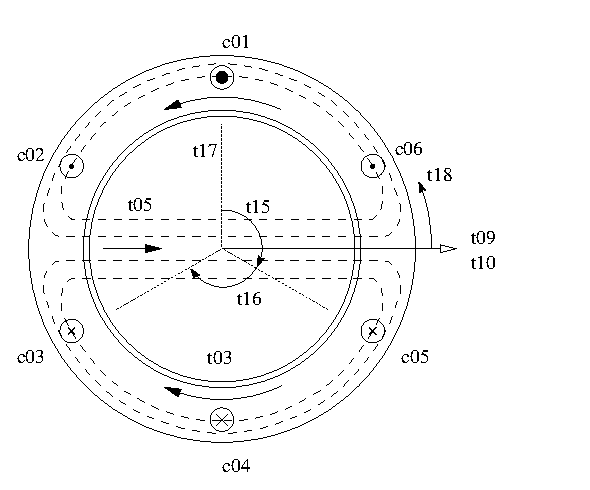
\includegraphics[height=5.3cm]{figs/f_mmf_2a.eps}
\end{psfrags}%}
  \hfill
  \subfloat[Spatial mmf distribution\label{fig:nt3mmf}]{
  \begin{psfrags}%
\psfragscanon

% text strings:
\psfrag{x01}{$0$}
\psfrag{x02}{$\frac{\pi}{3}$}
\psfrag{x03}{$\frac{2\pi}{3}$}
\psfrag{x04}{$\pi$}
\psfrag{x05}{$\frac{4\pi}{3}$}
\psfrag{x06}{$\frac{5\pi}{3}$}
\psfrag{x07}{$2\pi$}

\psfrag{c01}[bc]{+1}
\psfrag{c02}{-2}
\psfrag{c03}{+3}
\psfrag{c04}[bc]{-1}
\psfrag{c05}{+2}
\psfrag{c06}{-3}
\psfrag{t03}{$\mu \rightarrow \infty$}
\psfrag{t05}{$F$}
\psfrag{t07}[br]{$\theta$}
\psfrag{t08}{$F_2$ envelope}
\psfrag{t09}{magnetic}
\psfrag{t10}{axis}
\psfrag{t11}{$F_1$}
\psfrag{t12}{$F_2$}
\psfrag{t13}{$F_3$}
\psfrag{t14}{phase belt}
\psfrag{t15}{$-\frac{2\pi}{3}$}
\psfrag{t16}{$-\frac{2\pi}{3}$}
\psfrag{t17}{$+\pi$}
\psfrag{t18}{$\theta^{+}$}

\psfrag{t19}{(a)}
\psfrag{t20}{(b)}

\psfrag{p01}{$p_1$}
\psfrag{p02}{$p_2$}
\psfrag{p03}{$p_3$}
\psfrag{p04}{$p_4$}

% Figure:
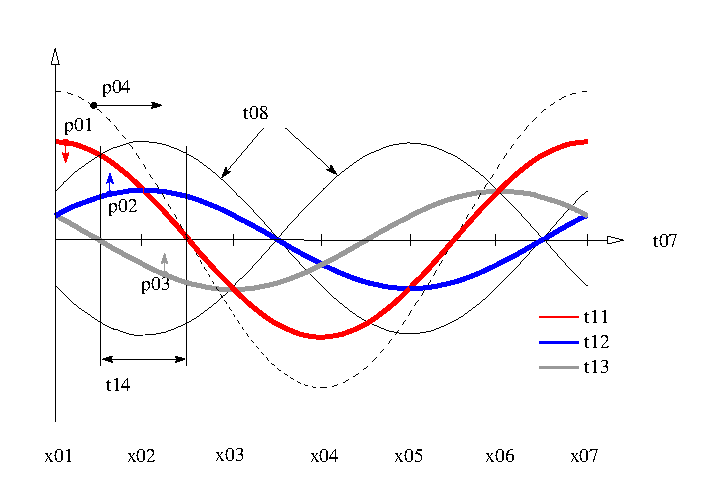
\includegraphics[height=5.3cm]{figs/f_mmf_2b.eps}
\end{psfrags}%}
  \caption{Three $N_t$-turn coils}
  \label{fig:mmf_2}
\end{figure}

Fig.~\ref{fig:mmf_2}\subref{fig:threecoils} shows graphically the mmf's of the three coils with $N_t$-turns. These are obtained by setting $m=3$ and applying the following three-phase currents 
\begin{equation}
  \label{eqn:3ph_i}
   i_n = \hat{I}\cos\left(\omega t +(n-1)\frac{2\pi}{m}\right),
  \qquad
  1 \leq n \leq m
\end{equation}
to the functions in \eqref{eqn:F_theta_t_3}. The resultant mmf will rotate in a counterclockwise direction. At $t=0$ $i_2=i_3=-\frac{1}{2}i_1$, meaning the mmf of $F_2$ and $F_3$ will be half of $F_1$. As time starts to increase, any point on $F_1$ will move downward while points on $F_2$ and $F_3$ will start moving in an upward direction. The points are marked $p_1$ through $p_3$ in the figure. Contrary to this, any point on the resultant mmf will start moving in the right direction (counter-clockwise) as indicated by point $p_4$. As time increases the resultant mmf rotates as shown in Fig.~\ref{fig:rotating_wave}. The fundamental mmf is shown at time equal to zero and a time instant $t=t_1$.
\begin{figure}
  \centering
  \fontsize{8}{0}\selectfont
  \subfloat[$t=0$\label{fig:mmfrot0}]{
  \begin{psfrags}%
\psfragscanon

% text strings:
\psfrag{t01}{+1}
\psfrag{t02}{-1}
\psfrag{t03}{+3}
\psfrag{t04}{-3}
\psfrag{t05}{+2}
\psfrag{t06}{-2}
\psfrag{t07}[bc]{$t=0$}
\psfrag{t08}[bc]{$t=t_1$}

% Figure:
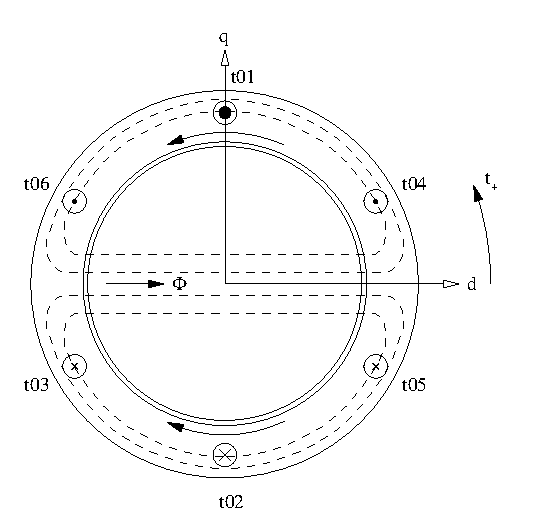
\includegraphics[height=6.2cm]{figs/f_mmf_rotationa.eps}
\end{psfrags}%}
  \hfill
  \subfloat[$t=t_1$\label{fig:mmfrot1}]{
  \begin{psfrags}%
\psfragscanon

% text strings:
\psfrag{t01}{+1}
\psfrag{t02}{-1}
\psfrag{t03}{+3}
\psfrag{t04}{-3}
\psfrag{t05}{+2}
\psfrag{t06}{-2}
\psfrag{t07}[bc]{$t=0$}
\psfrag{t08}[bc]{$t=t_1$}

% Figure:
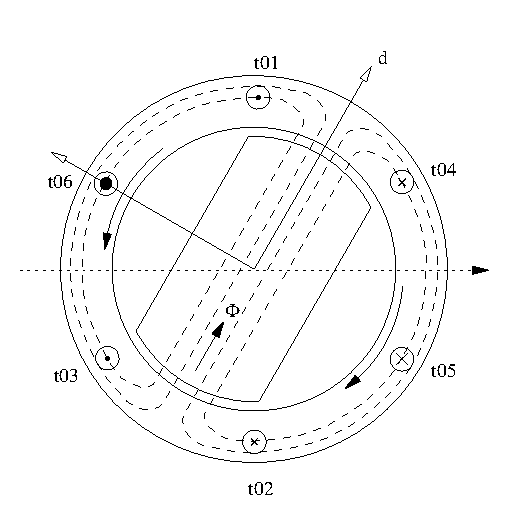
\includegraphics[height=6cm]{figs/f_mmf_rotationb.eps}
\end{psfrags}%}
  \caption[Rotation of the resultant mmf]{Rotation of the resultant mmf by displacing~%
  the three positive coil sides along the stator periphery}
  \label{fig:rotating_wave}
\end{figure}

\subsection{Definition of the mmf envelope functions}\label{subsec:mmf_def}
As time continues, any point on the standing wave will have a minimum and maximum value between which it oscillates. If $p_2$ is used as an example, it will be bounded as shown in Fig.~\ref{fig:mmf_2}\subref{fig:mmfrot1}, thus forming an envelope. Similarly, the remaining phases will each form envelope functions. The bounding functions for all the phases are given by
\begin{equation}
  \label{eqn:f_bound}
  f_n(\theta) = \hat{F_n}\cos\left[\theta+\frac{2\pi}{m}(n-1) \right], 
  \quad 1 \leq n \leq m
\end{equation}
and the mmf of any of the phases will be bounded, i.e. 
\begin{equation}
  -\left|f_n(\theta)\right| \leq F_n(\theta ,t) \leq \left|f_n(\theta)\right|
\end{equation}

\subsection{Phase belt definition}\label{subsec:phasebelt_def}
The mmf envelope functions in section \ref{subsec:mmf_def} allow the definition of the phase belt in a unique way, which make it possible to allocate the stator slots that belong to a phase before the coil sides are assigned. 
\begin{defth}
In general, the interval $\left\langle \theta_1,\theta_2 \right\rangle$ for which any of the $m$ bounding functions in \eqref{eqn:f_bound} is greater than the remaining $(m-1)$ functions is defined as a phase belt, i.e. 
\begin{equation}
 \left|f_i(\theta)\right| > \left|f_n(\theta)\right|, \quad
 \begin{cases}
   1 \leq n \leq m \\
   n \neq i
 \end{cases}
\end{equation}
and the interval $\left\langle \theta_1,\theta_2 \right\rangle$ spans $\frac{2\pi}{2m}$ radians. 
\end{defth}
A useful parameter to define is the total number of phase belts around the air gap periphery, i.e. 
\begin{equation}
  \label{eqn:Np}
  N_p = \frac{2\pi p}{\left(\frac{2\pi}{2m}\right)}=p\cdot2m
\end{equation}
and means that the phase belt sequence (for three phases) given in \eqref{eqn:phasebelt_sequence} repeat itself $p$ times around the air gap periphery.

\subsection{Higher order harmonics}
A similar procedure as for the working harmonic can be used to derive the direction of rotation for the higher order harmonics. The decomposition of the air gap mmf means that the resultant mmf is the sum of an infinite number of rotating waves. The general expression for harmonic order (for three phases and six phase belts) of the air gap mmf harmonics is
\begin{equation}
  \label{eqn:harm_oder}
  \nu = 1+6g \quad g=0,\mp1,\mp2,\ldots
\end{equation}
and the speed of rotation is given by 
\begin{equation}
  \omega_{\nu} = \frac{\omega}{\nu}
\end{equation}
A positive value of $\nu$ means that the harmonic is rotating counter-clockwise and a negative $\nu$ means it rotates clockwise. This convention is valid for the coil arrangement as given in Fig.~\ref{fig:mmf_2}(a) and the currents in \eqref{eqn:3ph_i}. The rotation speed is proportional to the inverse of the harmonic order.